\subsection{AST builder}
\label{sec:5-6-ast-builder}

\texttt{ANTLR} offre due diversi approcci per analizzare l'albero di parsing:
\begin{itemize}
    \item \textit{listener}: i metodi implementati per l'analisi dei nodi sono chiamati seguendo la ricerca
          in profondità (\textit{DFS, depth-first search});
    \item \textit{visitor}: i nodi possono essere visitati arbitrariamente tramite il metodo \texttt{visit},
          senza seguire un ordine specifico; non tutti i metodi devono essere implementati
          ed è possibile ignorare dei nodi o ri-visitarli.
\end{itemize}

\noindent La seconda opzione è indubbiamente più versatile, e può essere per esempio anche utilizzata
qualora si desideri evitare completamente la costruzione di un \textbf{AST} e chiamare i metodi di visita
per eseguire il codice (e.g. linguaggi interpretati).

\noindent Nel caso di \textbf{Funx-jt} la scelta ricade appunto sul \textit{visitor} in virtù
della probabilità di dover "saltare" alcuni nodi e ottenere direttamente le informazioni interne.

\noindent Durante la compilazione del progetto \texttt{Java}, \texttt{Gradle} è configurato per generare
le seguenti classi nel package \texttt{com.github.massimopavoni.funx.jt.parser}:
\begin{itemize}
    \item \texttt{FunxLexer}: \textit{lexer};
    \item \texttt{FunxParser}: \textit{parser};
    \item \texttt{FunxParserVisitor}: interfaccia generica per differenti implementazioni del \textit{visitor}
          (estende l'interfaccia \texttt{ParseTreeVisitor} di \texttt{ANTLR});
    \item \texttt{FunxParserBaseVisitor}: classe predefinita che percorre l'intero albero di parsing
          (estende la classe astratta \texttt{AbstractParseTreeVisitor} per ereditare alcuni metodi standard come \texttt{visitChildren}).
\end{itemize}

\noindent La classe \texttt{ASTBuilder} estende a sua volta \texttt{FunxParserBaseVisitor} e sovrascrive quasi tutti i metodi ereditati;
in particolare, \texttt{ASTBuilder} effettua la composizione degli schemi di tipo definiti dall'utente (sezione~\ref{sec:5-8-system-hm})
e l'eliminazione dello zucchero sintattico mediante l'uso di alcune proprietà e metodi ausiliari.


Inoltre, all'interno del package \texttt{com.github.massimopavoni.funx.jt.ast} viene definita una classe enumeratore,
\texttt{PreludeFunction}, contenente le funzioni di libreria standard, con i relativi simboli e gli schemi di tipo corrispondenti.

\vspace{4mm}
\begin{lstlisting}[caption={Parte del codice di \texttt{PreludeFunction}}, style=javaCode, label={lst:5-6-preludefunction-java}]
public enum PreludeFunction {
    COMPOSE(".", "compose",
        new Scheme(Set.of(0L, 1L, 2L),
            arrowOf(arrowOf(ZERO, ONE), arrowOf(TWO, ZERO), TWO, ONE)), false);

    public final String symbol;
    public final String id;
    public final Scheme scheme;
    public final boolean nativeJava;

    PreludeFunction(String symbol, String id,
        Scheme scheme, boolean nativeJava) { ... }

    public static PreludeFunction fromSymbol(String symbol) {
        return Utils.enumFromField(PreludeFunction.class,
            f @-> f.symbol.equals(symbol));
    }
}
\end{lstlisting}

\newpage

\begin{lstlisting}[caption={Metodi per astrazioni annidate e operatori simbolici binari}, style=javaCode, label={lst:5-6-auxiliary-methods-java}]
private ASTNode createLambdaChain(
        InputPosition position, Deque@<String@> params, ASTNode expression) {
    if (params.size() == 1)
        return new Expression.Lambda(
            position,
            params.getFirst(),
            expression);
    return new Expression.Lambda(
        position,
        params.pop(),
        createLambdaChain(position, params, expression));
}

private ASTNode binarySymbolApplication(
        InputPosition position, String symbol, ASTNode left, ASTNode right) {
    return new Expression.Application(
        position,
        new Expression.Application(
                position,
                new Expression.Variable(
                        position,
                        PreludeFunction.fromSymbol(symbol).id),
                left),
        right);
}
\end{lstlisting}
\vspace{4mm}
\begin{lstlisting}[caption={Alcuni metodi \texttt{visit} di \texttt{ASTBuilder}}, style=javaCode, label={lst:5-6-astbuilder-java}]
public class ASTBuilder extends FunxParserBaseVisitor@<ASTNode@> {
    @Override
    public ASTNode visitAppExpression(FunxParser.AppExpressionContext ctx) {
        return new Expression.Application(getInputPosition(ctx),
            visit(ctx.expression(0)),
            visit(ctx.expression(1)));
    }

    @Override
    public ASTNode visitComposeExpression(FunxParser.ComposeExpressionContext ctx) {
        return binarySymbolApplication(getInputPosition(ctx),
            Utils.fromLexerToken(ctx.bop.getType()),
            visit(ctx.expression(0)),
            visit(ctx.expression(1)));
    }
    
    @Override
    public ASTNode visitOrExpression(FunxParser.OrExpressionContext ctx) {
        // transform logical disjunction into if statement for lazy behavior
        return new Expression.If(getInputPosition(ctx),
            visit(ctx.expression(0)),
            new Expression.Constant(InputPosition.UNKNOWN, true),
            visit(ctx.expression(1)));
    }

    @Override
    public ASTNode visitLambda(FunxParser.LambdaContext ctx) {
        // lambda params are syntactic sugar for a lambda chain
        return createLambdaChain(getInputPosition(ctx),
            ctx.lambdaParams().VARID().stream().map(ParseTree::getText)
                    .collect(Collectors.toCollection(ArrayDeque::new)),
                visit(ctx.statement()));
    }
}    
\end{lstlisting}

\newpage

\noindent Il codice del compilatore include una classe astratta \texttt{ASTVisitor} atta a permettere l'analisi
dell'\textbf{AST} in modo simile ai \textit{visitor} di \texttt{ANTLR}.
Il Codice~\ref{lst:5-6-ast-example-funx} e la Figura~\ref{fig:5-6-ast-example-debug-graphviz}
mostrano un \textbf{AST} come verrebbe creato da \texttt{ASTBuilder}; la \textit{CLI} sviluppata fornisce
delle opzioni per la visualizzazione dell'albero, generata utilizzando il software \texttt{Graphviz}%
\footnote{Graph Visualization Software (\url{https://graphviz.org})}
con un \textit{visitor} (\texttt{GraphvizBuilder}) che scrive una stringa nel linguaggio \texttt{DOT}.

\vspace{4mm}
\begin{lstlisting}[caption={Programma in \textbf{Funx}}, style=funxCode, label={lst:5-6-ast-example-funx}]
tautology : Bool @-> Bool
tautology x = x || !!x
\end{lstlisting}

\begin{figure}
    \vspace{4mm}
    \begin{minipage}[c]{0.6\textwidth}
        \centering
        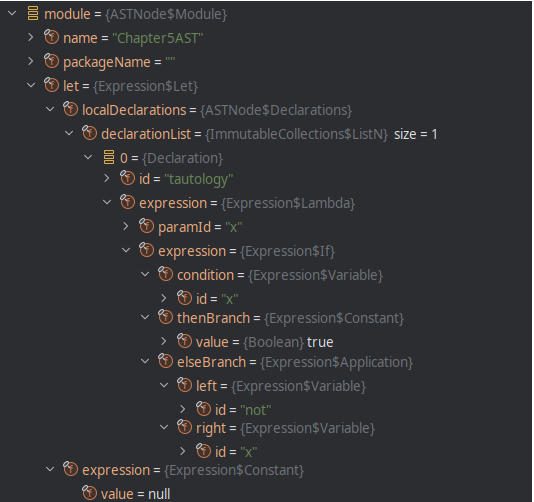
\includegraphics[width=\linewidth,height=\linewidth]{5-6-ast-example-debug.png}
    \end{minipage}%
    \hfill
    \begin{minipage}[c]{0.4\textwidth}
        \centering
        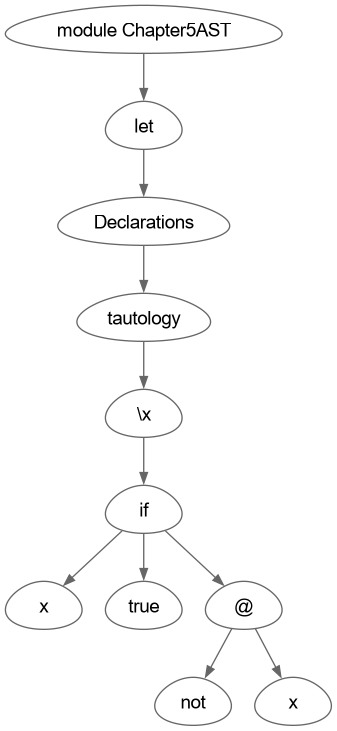
\includegraphics[width=0.8\linewidth]{5-6-ast-example-graphviz.png}
    \end{minipage}
    \caption{Oggetto \textbf{AST} in \textit{debug} e visualizzazione dell'albero}
    \label{fig:5-6-ast-example-debug-graphviz}
\end{figure}